\chapter{Качественное решение ДУ. Поле направлений}

\begin{figure}[h]
    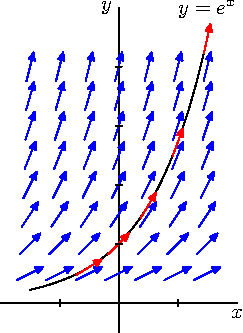
\includegraphics{fig1-1.pdf}
    \centering
    \caption{1-й скрипт}
\end{figure}

\section*{1-ый скрипт}
\verbatiminput{fig1.mp}

\begin{figure}[h]
    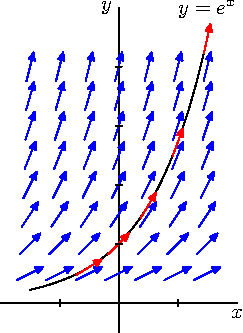
\includegraphics{myfig1-1.pdf}
    \centering
    \caption{Переписанный 1-ый скрипт}
\end{figure}

\section*{Переписанный 1-ый скрипт}
\verbatiminput{myfig1.mp}

\begin{figure}[h]
    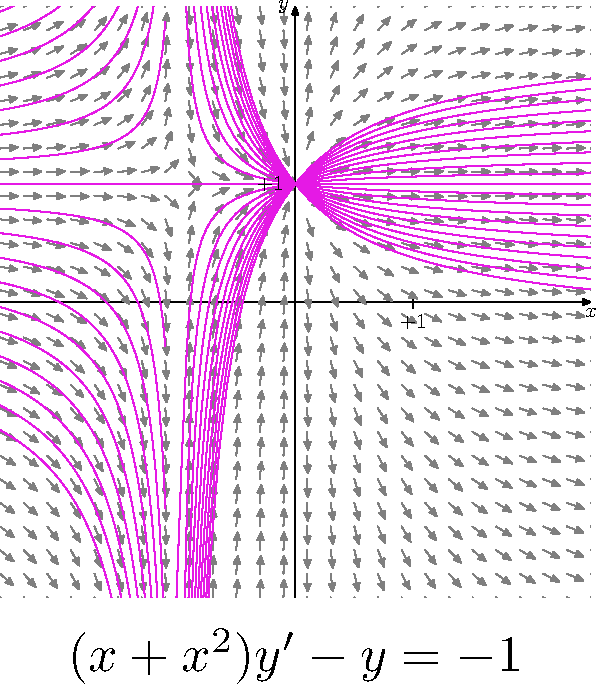
\includegraphics{fig2-1.pdf}
    \centering
    \caption{2-й скрипт}
\end{figure}

\section*{2-ый скрипт}
\verbatiminput{fig2.mp}

\begin{figure}[h]
    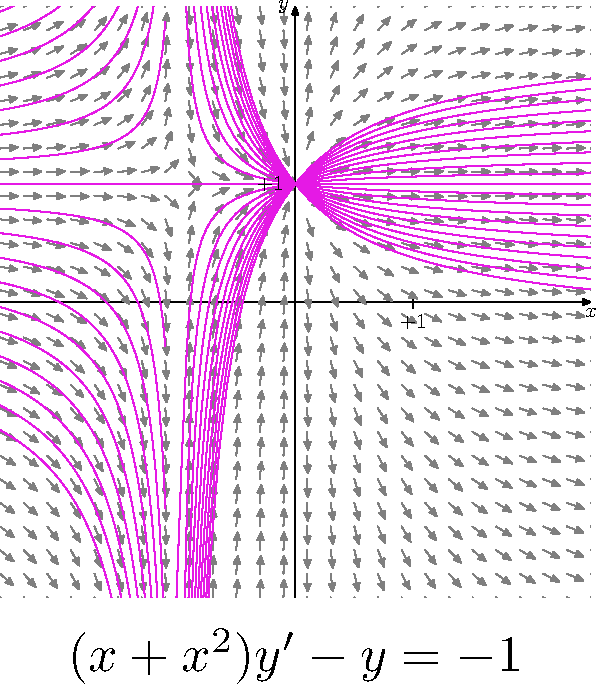
\includegraphics{myfig2-1.pdf}
    \centering
    \caption{Переписанный 2-ый скрипт}
\end{figure}

\section*{Переписанный 2-ый скрипт}
\verbatiminput{myfig2.mp}

\chapter{3d чертежи с использованием MetaPost (Asymptote, Ps-Tricks)}

\begin{figure}[h]
    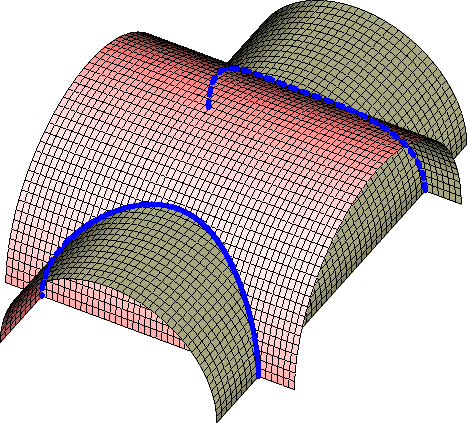
\includegraphics{fig3-1.pdf}
    \centering
    \caption{Intersection de deux demi-cylindres}
\end{figure}

\begin{figure}[h]
    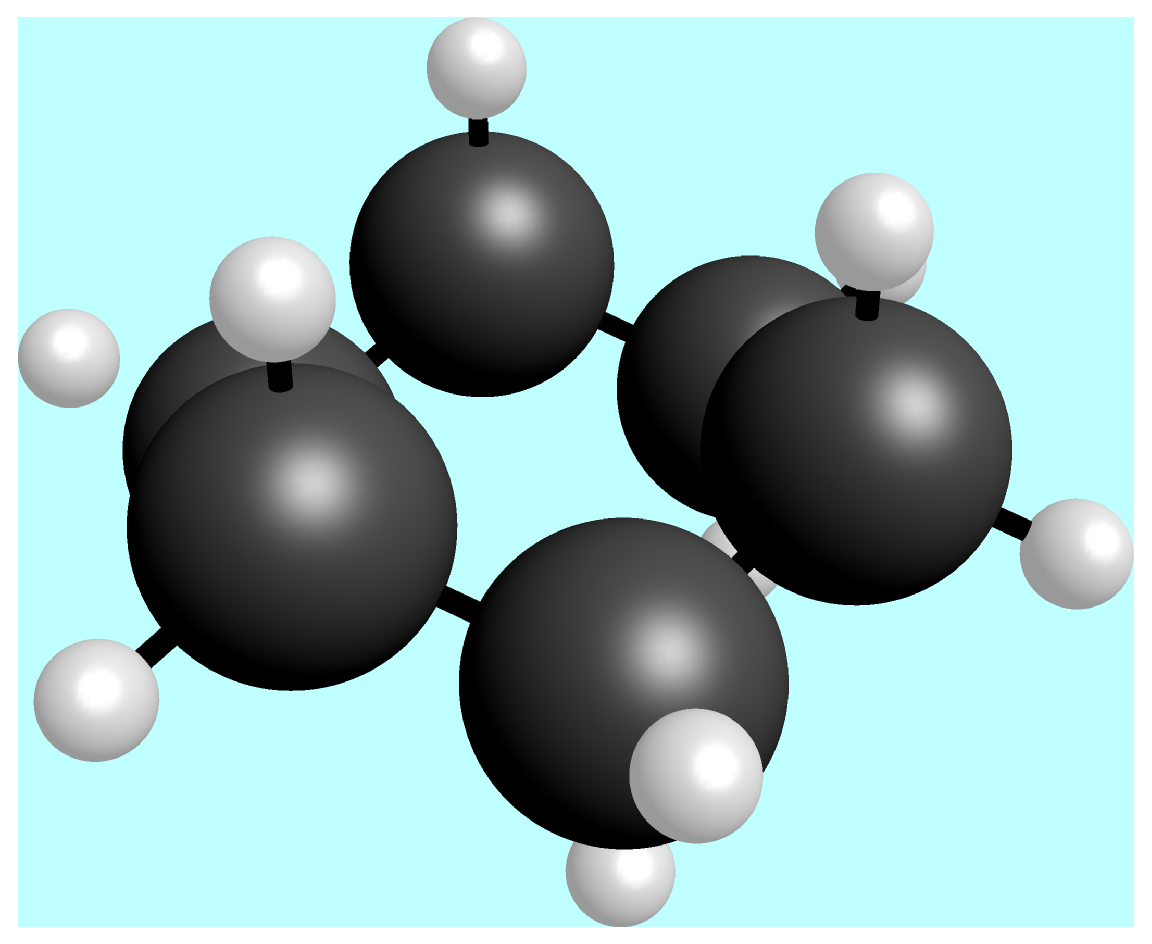
\includegraphics{script3}
    \centering
    \caption{3-й скрипт}
\end{figure}

\begin{figure}[h]
    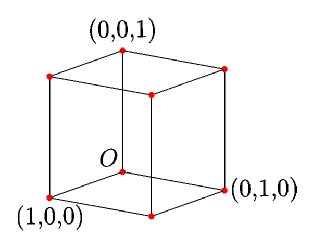
\includegraphics{myscript}
    \centering
    \caption{Трехмерный чертеж}
\end{figure}

\begin{figure}[h]
    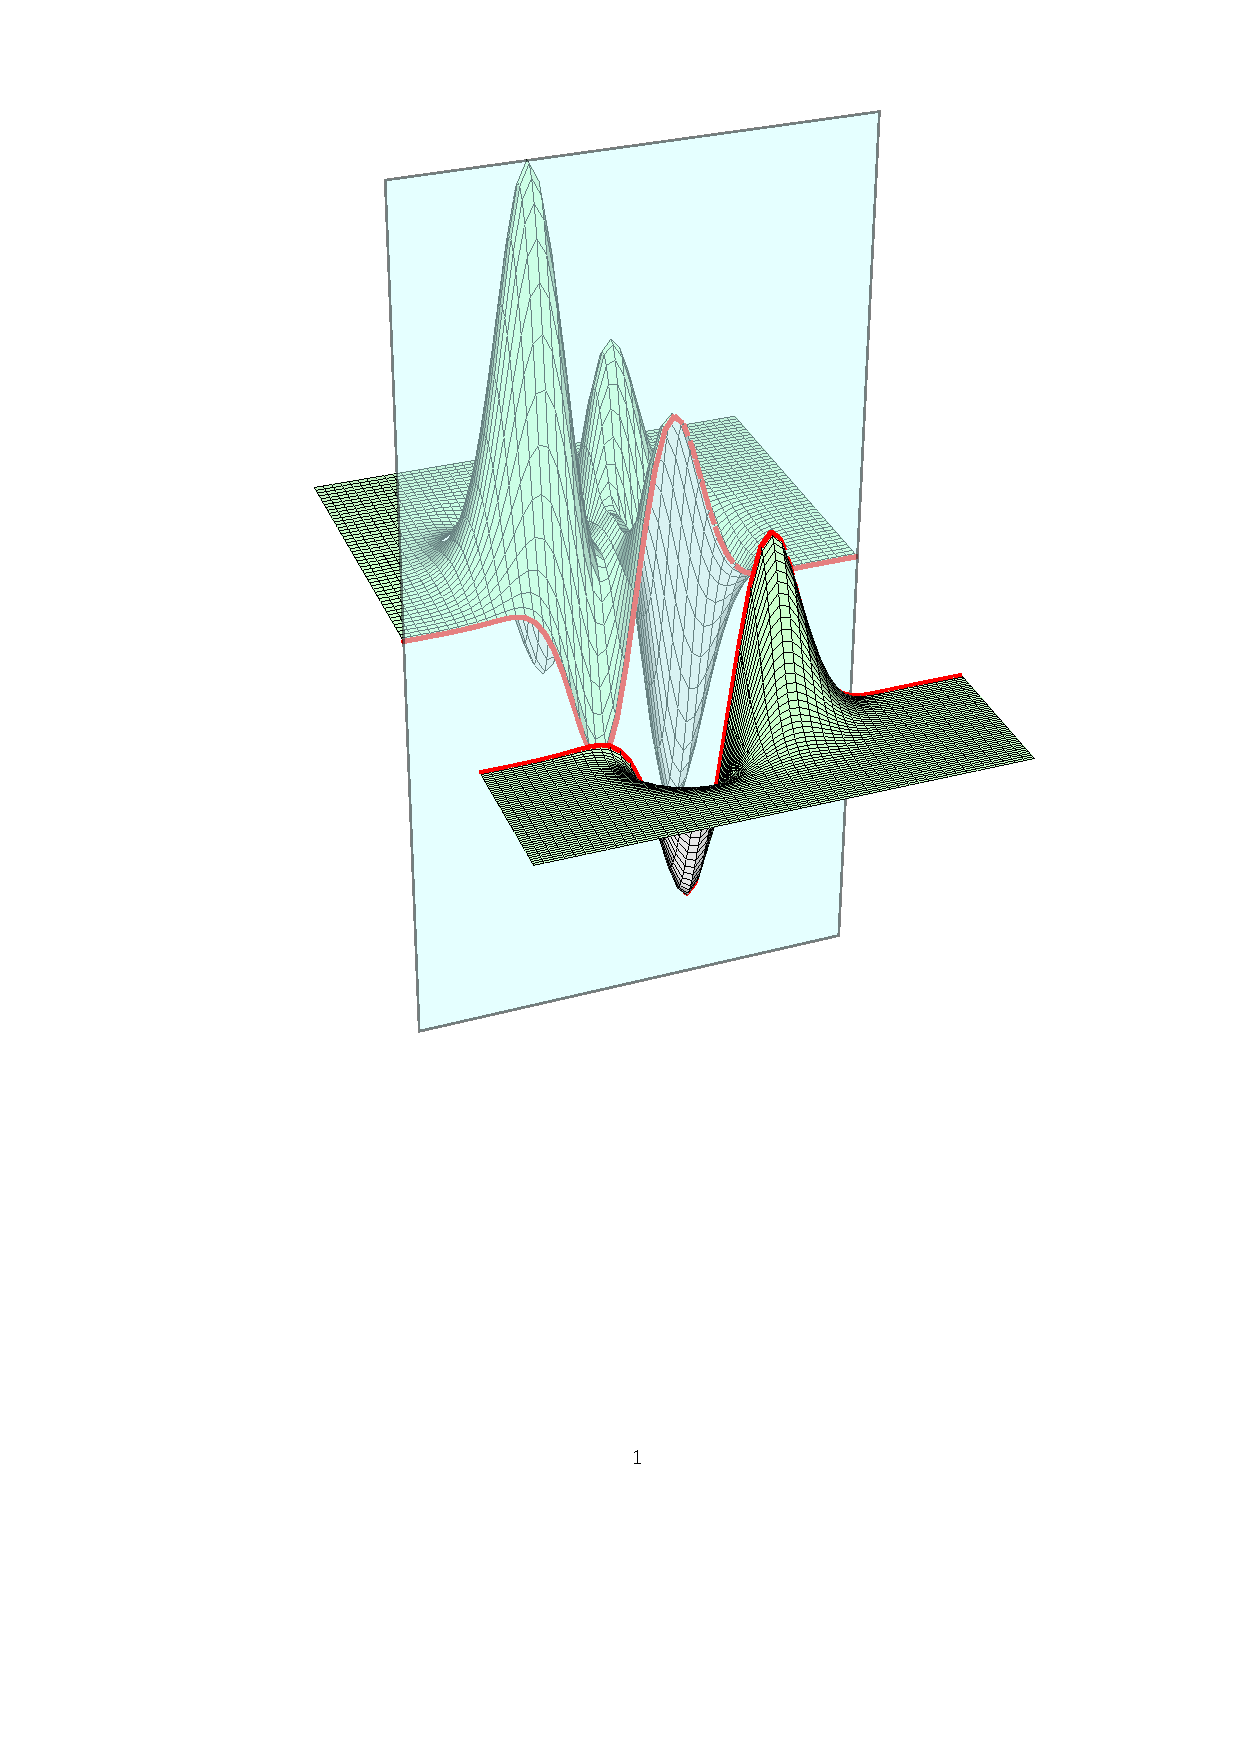
\includegraphics{script5.pdf}
    \centering
    \caption{PsTricks}
\end{figure}

\chapter{Вывод}

Картинки можно рисовать словами\cite{mpost} \cite{mpost_2}!

\bibliographystyle{gost780u}
\bibliography{main}
